\documentclass[11pt]{article}
\usepackage[left=3cm,right=3cm,top=3cm,bottom=3cm]{geometry} % page settings
\usepackage{float}
\usepackage{natbib}

\setcitestyle{round,aysep={}}

\setcounter{secnumdepth}{4}
\setcounter{tocdepth}{4}

\usepackage{amsmath}
\usepackage{amsthm, thmtools}
\usepackage{amssymb}
\usepackage{bm}
\usepackage{graphicx}   
\usepackage{enumitem}
\usepackage{listings}
\usepackage[hidelinks]{hyperref}
%\numberwithin{equation}

\usepackage{pgfplots}
\usepackage{tikz}
\usetikzlibrary{calc}
\usetikzlibrary{arrows.meta}
\usetikzlibrary{arrows}
\usepackage[makeroom,samesize]{cancel}

\usepackage{
nameref,
%\nameref
hyperref,
%\autoref
% n.b. \Autoref is defined by thmtools
cleveref,
% \cref
% n.b. cleveref after! hyperref
}

\usepackage{setspace}
\usepackage{lineno}
\title{No robust coexistence in a canonical model of plant-soil feedbacks}

\date{}
\author{Zachary R. Miller$^{1*}$ (zachmiller@uchicago.edu), Pablo Lech\'{o}n-Alonso$^{1}$ (plechon@uchicago.edu),\\ and Stefano Allesina$^{1,2}$ (sallesina@uchicago.edu) \\
	\\
	\normalsize{$^{1}$Department of Ecology \& Evolution, University of Chicago, Chicago, IL, USA}\\
	\normalsize{$^{2}$Northwestern Institute on Complex Systems, Evanston, IL, USA}\\
	\\
	\normalsize{*corresponding author (mailing: 1101 E. 57th Street, Chicago, IL 60637; phone: 484-331-4593)}\\
}


\begin{document}
	
\maketitle
\setstretch{1.5}

\noindent Running title: No coexistence in a plant-soil feedback model\\
Keywords: plant-soil feedbacks, legacy effects, coexistence, Bever model, bimatrix games, replicator equation \\

\noindent Author contributions: ZRM and SA performed the mathematical analysis, and PLA implemented the numerical simulations. ZRM wrote the manuscript, and all authors edited and discussed the text. \\

\noindent Data accessibility: Code for reproducing the numerical simulations is available at [ADD REPOSITORY].\\

\noindent Article type: Letter\\
Number of words in abstract: 137\\
Number of words in main text: \\
Number of references: 51 \\
Number of figures: 3

\linenumbers

\begin{abstract}
Plant-soil feedbacks (PSFs) are thought to represent a crucial mechanism generating frequency dependent dynamics in plant communities. Negative feedbacks, in particular, are routinely invoked to explain coexistence and the maintenance of diversity in species-rich communities. However, the primary modeling framework used to study PSFs considers only two plant species, and we lack clear theoretical expectations for how these complex interactions play out in communities with natural levels of diversity. Here, we demonstrate that this canonical model for PSFs is equivalent to a well-studied model from evolutionary game theory, and using this equivalence, we are able to characterize the dynamics with an arbitrary number of plant species. Surprisingly, we find that coexistence of more than two species is virtually impossible in this model, suggesting that alternative theoretical frameworks are needed to describe feedbacks observed in diverse natural communities. 
\end{abstract}

\section{Introduction}

It has become well understood that reciprocal interactions between plants and the soil biota, known as plant-soil feedbacks (PSFs), play an important role in structuring the composition and dynamics of plant communities. PSFs operate alongside other factors, including abiotic drivers \citep{bennett2019mechanisms} and above-ground trophic interactions \citep{van2009empirical}, but are thought to be a key mechanism generating negative frequency-dependent feedbacks that promote coexistence and maintain plant diversity \citep{kulmatiski2008plant,van2013plant,bever2015maintenance}. The existence of PSFs has long been known \citep{van1993plant,bever1994feedback}, but our understanding of their importance -- particularly in relation to patterns of coexistence -- has developed rapidly in recent years \citep{klironomos2002feedback,petermann2008janzen,mangan2010negative}. Broad interest in PSFs was ignited by the development of simple mathematical models, which illustrated the potential of PSFs to mediate plant coexistence \citep{bever1997incorporating,bever2003soil,ke2015incorporating}. These models have played a guiding role for a wide range of empirical studies, as well \citep{kulmatiski2008plant,kulmatiski2011testing,pernilla2010plant}.

The first, and still most widely known and used, model for PSFs was introduced by Bever and colleagues in the 1990s \citep{bever1992ecological,bever1997incorporating,bever1999dynamics,bever2003soil}. In this framework, often referred to simply as the Bever model, each plant species is assumed to promote the growth of a specific soil component (i.e. associated bacteria, fungi, invertebrates, considered collectively) in the vicinity of individual plants. In turn, the fitness of each plant species is impacted by the relative frequency of different soil components. Starting from minimal assumptions, \citet{bever1997incorporating} derived a set of differential equations to capture these dynamics. PSFs can be either positive (fitness of a plant species is increased by its corresponding soil component) or negative (a plant species experiences lower relative fitness in its own soil). Bever \textit{et al.} introduced a single quantity to summarize whether community-wide PSFs are positive or negative, and showed that this value characterizes the dynamical behavior of the model. In the original Bever model of two plant species, positive PSFs lead to exclusion of one species, while negative PSFs result in neutral oscillations. It is thus widely suggested that negative PSFs help sustain coexistence in real-world plant communities \citep{kulmatiski2008plant,van2013plant}, perhaps with spatial asynchrony playing a role in stabilizing the cyclic dynamics \citep{revilla2013plant,bever2003soil}.

Subsequent studies have generalized this model to include, for example, more realistic functional forms \citep{umbanhowar2005simple, eppinga2006accumulation}, more explicit representations of the soil community \citep{bever2010rooting}, spatial structure \citep{eppinga2006accumulation,molofsky2002negative,suding2013consequences}, or additional processes such as direct competitive interactions between plants \citep{bever2003soil}. However, the original Bever model remains an important touchstone for the theory of PSFs \citep{ke2015incorporating,ke2020effects}, and informs empirical research through the interaction coefficient, $I_s$, derived by Bever \textit{et al.}, which is commonly measured and used to draw conclusions about coexistence in experimental studies. Despite the ubiquity of this model, and the fruitful interplay of theory and experiment in the PSF literature, extensions to communities with more than two or three species have appeared only rarely and recently \citep[but see][]{eppinga2018frequency,mack2019plant}. While PSF models motivate hypotheses and conclusions about species-rich natural communities, there is much still unknown about the behavior of these models with natural levels of diversity \citep{van2013plant}.

Here, we extend the Bever model to include any number of plant species, and show that the model is equivalent to a special form of the replicator equation studied in evolutionary game theory \citep{hofbauer1998evolutionary}. In particular, this model corresponds to the class of bimatrix games, where there are two players (here, plants and soil components) which interact with asymmetric strategies and payoffs. The replicator dynamics of bimatrix games are well-studied, allowing us to characterize many properties of the Bever model with $n$ plant species. Surprisingly, using this equivalence, we show that coexistence of more than two species in this model is never robust. 

\section{Results}

\subsection{Generalizing a classic PSF model}

Inspired by emerging empirical evidence for the important role of PSFs in plant community dynamics and coexistence \citep{van1993plant,bever1994feedback}, \citet{bever1997incorporating} introduced a simple mathematical model to investigate their behavior. In this model, two plant species, $1$ and $2$, grow exponentially with growth rates determined by the state of the soil biota in the system. These effects of soil on plants are specified by parameters $\alpha_{ij}$, the growth rate of plant species $i$ in soil type $j$. There is a soil component corresponding to each plant species, which grows exponentially in the presence of its associated plant at a rate $\beta_i$. Bever \textit{et al.} set an important precedent by considering dynamics of \emph{relative} abundances in such a system; starting from dynamics of the form

\begin{align} \label{2spp_absolute}
	\begin{cases}
	\frac{dx_i}{dt} &= x_i \left( \frac{\alpha_{ii} \, y_i + \alpha_{ij} \, y_j}{y_i + y_j} \right) \, , \quad  i, j = 1,2 \\
	\frac{dy_i}{dt} &= y_i \left( \frac{\beta_i \, x_i}{x_i + x_j} \right)
	\end{cases}
\end{align}
for the \emph{absolute} abundances of plants ($x_i$) and soil components ($y_i$), one considers the relative abundances (frequencies), $p_i = x_i \, / \sum_j x_j$ and $q_i = y_i \, / \sum_{j} y_j$. The dynamics for these frequencies are easily derived from Eq.~\ref{2spp_absolute}, and using the facts $p_i = 1 - p_j$ and $q_i = 1 - q_j$, can be written as:

\begin{align} \label{2spp_relative}
\begin{cases}
\frac{dp_i}{dt} &= p_i \, p_j \left( (\alpha_{ii} - \alpha_{ji}) \, q_i + (\alpha_{ij} - \alpha_{jj}) \, q_j \right) \, , \quad  i, j = 1,2 \\
\frac{dq_i}{dt} &= q_i \, q_j (\beta_i \, p_i - \beta_j \, p_j) \, .
\end{cases}
\end{align}
This model may admit a coexistence equilibrium where

\begin{align} \label{2spp_eq}
\begin{cases}
p_i^\star &= \frac{\beta_j}{\beta_i + \beta_j} \, , \quad  i, j = 1,2 \\
q_i^\star &= \frac{\alpha_{jj} - \alpha_{ji}}{\alpha_{ii} - \alpha_{ij} + \alpha_{jj} - \alpha_{ji}} \, .
\end{cases}
\end{align}

A central finding of the analysis by Bever \textit{et al.} was that the denominator of $q_i^*$, which they termed the ``interaction coefficient'', $I_s$ ($= \alpha_{ii} - \alpha_{ij} + \alpha_{jj} - \alpha_{ji}$), controls the model dynamics: When $I_s > 0$, which represents a community with positive feedbacks, the equilibrium in Eq.~\ref{2spp_eq} is unstable, and the two species cannot coexist. On the other hand, when $I_s < 0$, the equilibrium is neutrally stable, and the dynamics cycle around it, providing a form of non-equilibrium coexistence. In fact, these conclusions depend on the existence of a feasible equilibrium (i.e. positive equilibrium values), which further requires that $\alpha_{ii} < \alpha_{ji}$, for both $i, j = 1, 2$, in order for the model to exhibit coexistence \citep{bever1997incorporating,ke2015incorporating}. 

This coexistence is fragile. Species frequencies oscillate neutrally, similar to the textbook example of Lotka-Volterra predator-prey dynamics. Any stochasticity, external forcing, or time variation in the model parameters can destroy these finely balanced oscillations and cause one species to go extinct \citep{revilla2013plant}. However, coupled with mechanisms that buffer the system from extinctions, such as migration between desynchronized patches or the presence of a seed bank, the negative feedbacks in this model might produce sustained coexistence \citep{revilla2013plant, bever2003soil}. 

Of course, most natural plant communities feature more than two coexisting species, and it is precisely in the most diverse communities where mechanisms of coexistence hold the greatest interest \citep{van2013plant}. While it is not immediately clear how to generalize Eq.~\ref{2spp_relative} to more than two species, Eq.~\ref{2spp_absolute} is naturally extended by maintaining the assumption that the overall growth rate for any plant is a weighted average of its growth rate in each soil type:

\begin{align} \label{nspp_absolute}
\begin{cases}
\frac{dx_i}{dt} &= x_i \left(\sum_{j} \alpha_{ij} \, q_j \right) \, , \quad  i = 1, \dots n \\
\frac{dy_i}{dt} &= y_i \left( \beta_i \, p_i \right) \, .
\end{cases}
\end{align}
From Eq.~\ref{nspp_absolute}, one can derive the $n$-species analogue of Eq.~\ref{2spp_relative} (Fig.~\ref{fig:concept}),

\begin{align} \label{nspp_relative}
\begin{cases}
\frac{dp_i}{dt} &= p_i \left(\sum_{j} \alpha_{ij} \, q_j - \sum_{j, k} \alpha_{jk} \, p_j \, q_k \right) \, , \quad  i = 1, \dots n \\
\frac{dq_i}{dt} &= q_i \left(\beta_{i} \, p_i - \sum_{j} \beta_{j} \, p_j \, q_j  \right) \,
\end{cases}
\end{align}
giving the dynamics for species and soil component frequencies. Eq.~\ref{nspp_relative} is conveniently expressed in matrix form as

\begin{align} \label{matrix_form}
\begin{cases}
\frac{d\bm{p}}{dt} &= D(\bm{p}) \left(A \bm{q} - (\bm{p}^T A \bm{q}) \bm{1} \right) \\
\frac{d\bm{q}}{dt} &= D(\bm{q}) \left(B \bm{p} - (\bm{q}^T B \bm{p}) \bm{1}  \right) \,
\end{cases}
\end{align}
where vectors are indicated in boldface (e.g. $\bm{p}$ is the vector of species frequencies $(p_1, p_2, \dots p_n)^T$ and $\bm{1}$ is a vector of $n$ ones) and $D(\bm{z})$ is the diagonal matrix with vector $\bm{z}$ on the diagonal. We have introduced the matrices $A = (\alpha_{ij})$ and $B = D(\beta_1, \beta_2, \dots \beta_n)$, specifying soil effects on plants and plant effects on soil, respectively. Because $\bm{p}$ and $\bm{q}$ are vectors of frequencies, they must sum to one: $\bm{1}^T \bm{p} = \bm{1}^T \bm{q} = 1$. Using these constraints, one can easily show that the Bever model (Eq.~\ref{2spp_relative}) is a special case of Eqs.~\ref{nspp_relative} and \ref{matrix_form} when $n = 2$.

\begin{figure*}
	\centering
	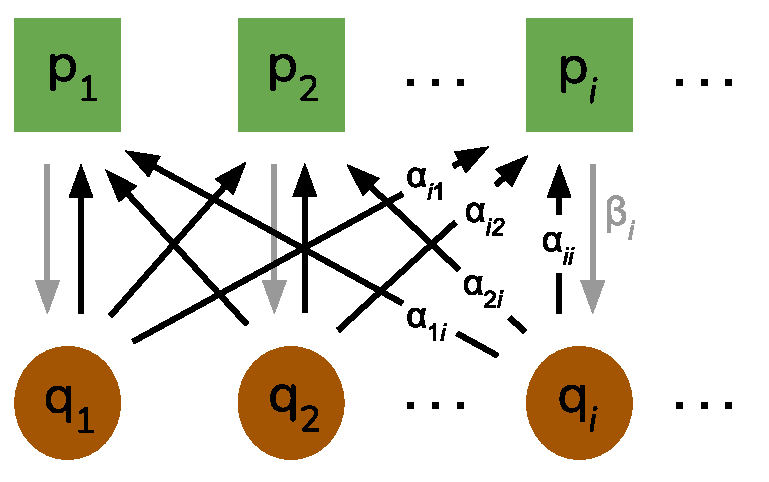
\includegraphics[width=\textwidth]{figure_1.pdf}
	\caption[Structure of the $n$-species Bever model]
	{The model described by Eqs.~\ref{nspp_relative}-\ref{matrix_form} is shown here graphically. Plant species (green squares) promote the growth of their respective soil components (brown circles) at a rate $\beta_i$ (gray arrows). In turn, growth of each plant is governed by the mix of soil components present in the system, with the effect of soil component $j$ on species $i$ quantified by the parameter $\alpha_{ij}$ (black arrows). This model is a straightforward extension of the model proposed by \citet{bever1997incorporating} to an arbitrary number of species. Note only selected parameter labels are shown for clarity.}
	\label{fig:concept}
\end{figure*}

\subsection{Equivalence to bimatrix game dynamics}

Systems that take the form of Eq.~\ref{matrix_form} are well-known and well-studied in evolutionary game theory. Our generalization of the Bever model is a special case of the \emph{replicator equation}, corresponding to the class of \emph{bimatrix games} \citep{taylor1979evolutionarily,hofbauer1996evolutionary,hofbauer1998evolutionary,cressman2014replicator}. Bimatrix games arise in diverse contexts, such as animal behavior \citep{taylor1979evolutionarily,selten1988note}, evolutionary theory \citep{hofbauer1998evolutionary,cressman2014replicator}, and economics \citep{friedman1991evolutionary}, where they model games with asymmetric players. In a bimatrix game, each player (here, the plant community and the soil) has a distinct set of strategies (plants species and soil components, respectively) and payoffs (realized growth rates).

Much is known about bimatrix game dynamics, and we can draw on this body of knowledge to characterize the behavior of the Bever model with $n$ species. Essential mathematical background and details are presented in the Supplemental Methods; for a detailed introduction to bimatrix games, see \citet{hofbauer1998evolutionary}.

Under the mild condition that matrix $A$ is invertible, Eq.~\ref{matrix_form} admits a unique coexistence equilibrium given by $\bm{p}^\star = k_p \, B^{-1} \bm{1}$ and $\bm{q}^\star = k_q \, A^{-1} \bm{1}$, where $k_p = 1 / (\bm{1}^T B^{-1} \bm{1})$ and $k_q = 1 / (\bm{1}^T A^{-1} \bm{1})$ are constants of proportionality that ensure the equilibrium frequencies sum to one for both plants and soil. Because $B$ is a diagonal matrix, and all $\beta_i$ are assumed positive, the equilibrium plant frequencies, $\bm{p}^\star$, are always positive, as well. Thus, feasibility of the equilibrium hinges on the soil frequencies, $\bm{q}^\star$, which are all positive if the elements of $A^{-1} \bm{1}$ all share the same sign.

As we have seen, when the community consists of two species, the coexistence equilibrium, if feasible, can be either unstable or neutrally stable. In fact, the same is true for the $n$-species extension  \citep[and, more generally, for any bimatrix game dynamics,][]{eshel1983coevolutionary,selten1988note,hofbauer1998evolutionary}. This can be established using straightforward local stability analysis, after accounting for the relative abundance constraints, which imply $p_n = 1 - \sum_{i = 1}^{n-1} p_i$ and $q_n = 1 - \sum_{i = 1}^{n-1} q_i$. Using these substitutions, Eq.~\ref{nspp_relative} can be written as a system of $2 n - 2$ (rather than $2 n$) equations, and the community matrix for this reduced model has a very simple form (see Supplemental Methods). In particular, due to the bipartite structure of the model, the community matrix has all zero diagonal elements, which implies that the eigenvalues of this matrix sum to zero. These eigenvalues govern the stability of the coexistence equilibrium, and this property leaves two qualitatively distinct possibilities: either the eigenvalues have a mix of positive and negative real parts (in which case the equilibrium is unstable), or the eigenvalues all have zero real part (in which case the equilibrium is neutrally stable). Already, we can see that the model never exhibits equilibrium coexistence, regardless of the number of species.

Another notable property of bimatrix game dynamics is that the vector field defined by the model equations is divergence-free or incompressible \citep[see][for a proof]{hofbauer1998evolutionary}. The divergence theorem from vector calculus \citep{arfken1985mathematical} then tells us that Eq.~\ref{matrix_form} cannot have any attractors -- that is, regions of the phase space that ``pull in'' trajectories -- with multiple species. This rules out coexistence in a stable limit cycle or other non-equilibrium attractors (e.g. chaotic attractors). Thus, only the relatively fragile coexistence afforded by neutral oscillations is possible, as in the two-species model.

Based on the local stability properties of the coexistence equilibrium, Bever \textit{et al.} concluded that such neutral cycles arise for two species when $\alpha_{11} < \alpha_{21}$ and $\alpha_{22} < \alpha_{12}$. The equivalence between their model and a bimatrix game with two strategies allows us to give a fuller picture of these cycles. Namely, we can identify a constant of motion for the two-species dynamics:

\begin{equation}
	H = (\alpha_{12} - \alpha_{22}) \log q_1 + (\alpha_{21} - \alpha_{11}) \log q_2 + \beta_2 \log p_1 + \beta_1 \log p_2 .
\end{equation} 
Using the chain rule and time derivatives in Eq.~\ref{2spp_relative}, it is easy to show that $\frac{dH}{dt} = 0$ for any plant and soil frequencies (see Supplemental Methods). The level curves of $H$ form closed orbits around the equilibrium when the equilibrium is neutrally stable. Thus, $H$ implicitly defines the trajectories of the model, and can be used to determine characteristics such as the amplitude of oscillations arising from particular initial frequencies.

Because neutral cycles provide the only possible form of coexistence in this model, a key question becomes whether and when neutral cycles with $n$ species can arise. Do the ``negative feedback'' conditions identified by Bever \textit{et al.} generalize in richer communities? Indeed, they do; however, for more than two species, these conditions are very severe. The model in Eq.~\ref{matrix_form} supports oscillations with $n$ species -- for any $n$ -- if matrices $A$ and $B$ satisfy a precise relationship (Fig.~\ref{fig:fragile}; see Supplemental Methods for details). In particular, the model parameters must satisfy the conditions $\alpha_{ij} = \gamma_i + \delta_j$ for some constants $\gamma_i, \delta_i$ in $i = 1, \dots, n$ (when $i \neq j$), and $\alpha_{ii} = \gamma_i + \delta_i- c \beta_i$ (where $c$ is a positive constant independent of $i$). In the language of bimatrix games, such systems are called \emph{rescaled zero-sum games} \citep{hofbauer1996evolutionary,hofbauer1998evolutionary}. It is a long-standing conjecture in evolutionary game theory that these parameterizations are the \emph{only} cases where $n$-species coexistence can occur \citep{hofbauer1996evolutionary,hofbauer2011deterministic}.

Ecologically, these conditions mean there is a fixed effect of each soil type and plant species identity, and the growth rate of plant $i$ in soil type $j$ is the additive combination of these two, with no interaction effects. The only exception is for plants growing in their own soil type, which must experience a fitness cost ($\gamma_i + \delta_i - \alpha_{ii}$) exactly proportional to the rate at which they promote growth of the soil type ($\beta_i$).  
These conditions clearly extend the intuitive notion that each plant must have a disadvantage in its corresponding soil type to allow coexistence. But the parameters of the model are constrained so strongly that we never expect to observe cycles with more than two species in practice. When $n > 2$, a great deal of fine-tuning is necessary to satisfy the conditions yielding a rescaled zero-sum game; the probability that random parameters will be suitable is infinitesimally small. We confirm this numerically with simulations shown in Fig.~\ref{fig:histograms}. Although $n$-species cycles are clearly possible (as in Fig.~\ref{fig:fragile}), for parameters drawn independently at random, communities always collapse to zero, one, or two species, regardless of the initial richness. 

Not only are parameter combinations permitting many-species oscillations rare, they are also extremely sensitive to small changes to the parameter values. The rescaled zero-sum condition imposes many exact equality constraints on the matrix $A$ (e.g. $\alpha_{ij} - \alpha_{ik} = \alpha_{lj} - \alpha_{lk}$ for all $i, j, k,$ and $l$). Even if mechanisms exist to generate the requisite qualitative patterns, inevitable quantitative variation in real-world communities will disrupt coexistence (Fig.~\ref{fig:fragile}). Coexistence of $n > 2$ species -- even in the weak sense of neutral cycles -- is not robust to small changes in the model parameters.

Interestingly, the two-species model is not subject to the same fragility. It can be shown (see Supplemental Methods) that all $2 \times 2$ bimatrix games take the same general form as a rescaled zero-sum game, although the constant $c$ may be positive or negative, depending on the parameters. When $I_s$, the interaction coefficient identified by Bever \textit{et al.}, is negative, $c$ is positive, ensuring (neutral) stability. This condition amounts to an inequality constraint, rather than an equality constraint, and so it \emph{is} generally robust to small variations in model parameters (Fig.~\ref{fig:fragile}). As we can now see, the case $n = 2$ is unique in this regard. 

\begin{figure*}
	\centering
	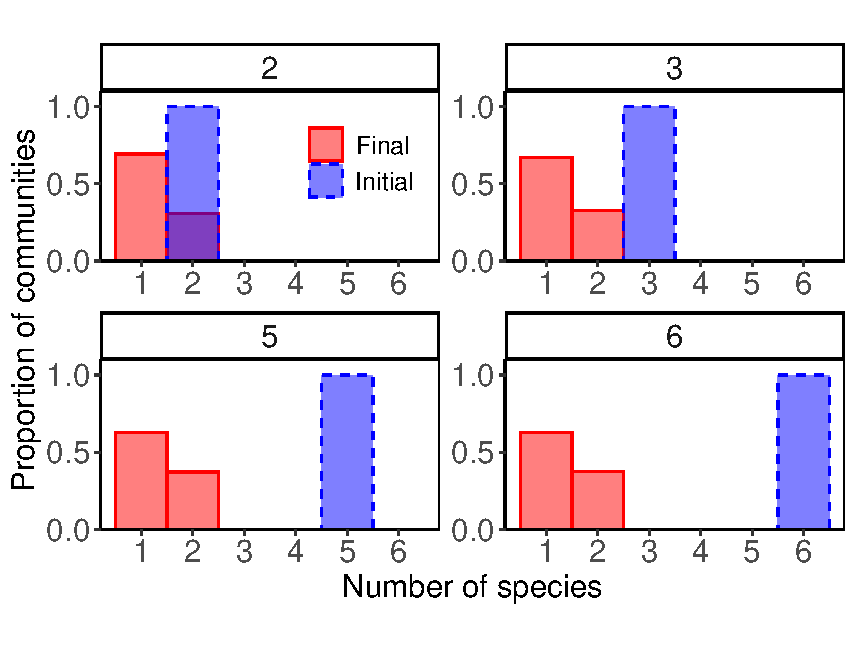
\includegraphics[width=\textwidth]{figure_2.pdf}
	\caption[Final community sizes with varying initial richness]
	{Final community sizes with varying initial richness. We show the distribution of final richness (number of species, in red) for 500 \textbf{(???)} communities governed by the $n$-species Bever model, initialized with 2, 3, 5, or 6 plant species. Parameters $\alpha_{ij}$ and $\beta_{i}$  were sampled independently from a standard uniform distribution, $U[0,1]$. For each random parameterization at each level of initial richness, we integrated the dynamics of Eq.~\ref{matrix_form} until the system reached a periodic orbit or until only one species remained. In agreement with the conjecture that coexistence of more than two species is vanishingly unlikely, we found that, regardless of the number of species initially present, every community collapsed to a subset of one or two surviving species.}
	\label{fig:histograms}
\end{figure*}


\begin{figure*}
	\centering
	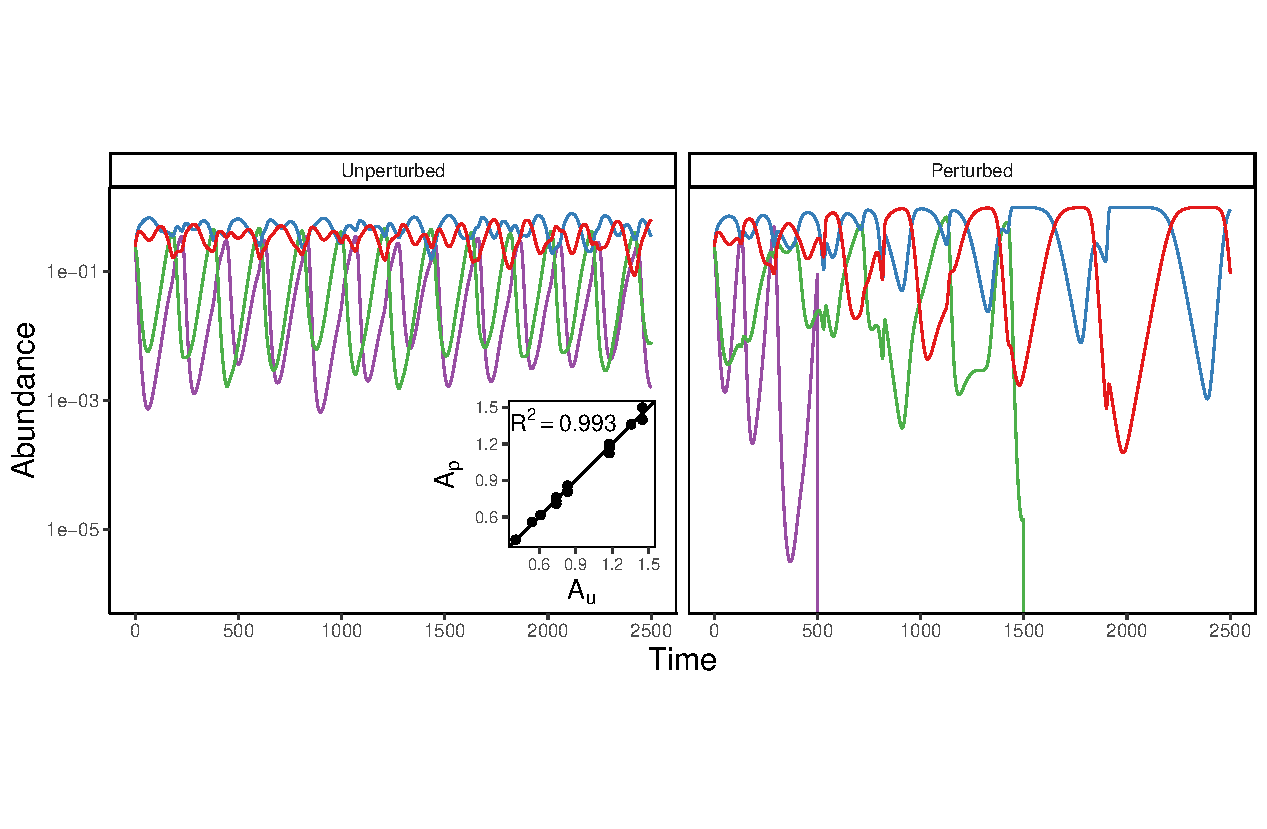
\includegraphics[width=\textwidth]{figure_3.pdf}
	\caption{Caption for Fig3}
	\label{fig:fragile}
\end{figure*}


\section{Discussion}

The Bever model has played a central role in motivating PSF research, and continues to guide both theory and experiment in this fast-growing field \citep{bever2015maintenance, kandlikar2019winning, ke2020effects}. Here, we extend the Bever model to any number of species, and highlight its equivalence to bimatrix game dynamics. Taking advantage of the well-developed theory for these dynamics, we are able to characterize the behavior of the generalized Bever model in detail.

Our central finding is that there can be no robust coexistence of plant species in this model. Regardless of the number of species, $n$, the model never exhibits equilibrium coexistence or other attractors. Coexistence can be attained through neutral oscillations, but these dynamics lack any restoring force and are easily destabilized by stochasticity or exogenous forcing. In this respect, the generalized model behaves similarly to the now-classic two-species system. However, unlike the two-species model, oscillations with $n > 2$ species can only result under very restricted parameter combinations. These parameterizations are vanishingly unlikely to arise by chance, and highly sensitive to small deviations. Thus, coexistence of more than two species is neither dynamically nor structurally stable.

This result may be surprising, because a significant body of experimental evidence indicates that PSFs can play an important role in mediating the coexistence of more than two species in natural communities \citep{kulmatiski2008plant,petermann2008janzen,mangan2010negative,bever2015maintenance}. Apparently, the picture suggested by the two-species Bever model generalizes in nature, but not in the model framework itself. We note that this framework was introduced as an intentional simplification to illustrate the potential role of PSFs in mediating coexistence, not to accurately model the biological details of PSFs. Indeed, the model has been wildly successfully in spurring research into PSFs. Alongside empirical study of these processes, other modeling approaches have emerged, accounting for more biological realism \citep[e.g.,][]{umbanhowar2005simple,eppstein2007invasiveness,bever2010rooting}, or with the demonstrated capacity to produce multispecies coexistence  \citep[e.g.,][]{bonanomi2005negative,miller2021metapopulations}. Some of these are minor modifications of the Bever model framework; others build on distinct foundations \citep{ke2015incorporating,ke2020effects}. Our results suggest that these various avenues are worth pursuing further.

Alternative modeling approaches are particularly important for better integration of theory and data. The predictions of the Bever model are commonly used to guide the design and analysis of PSF experiments, especially in drawing conclusions about coexistence. Our analysis cautions that applications of this model in multispecies communities might lead to incorrect inference. For example, attempts to parameterize the Bever model for three species using empirical data have produced predictions of non-coexistence in plant communities that coexist experimentally \citep{kulmatiski2011testing}. In many other studies, the pairwise interaction coefficient, $I_s$, is calculated for species pairs and used to assess whole-community coexistence \citep{kulmatiski2008plant,fitzsimons2010importance,pendergast2013belowground,suding2013consequences,kuebbing2015plant,smith2015plant,bauer2017effects,kandlikar2019winning}. However, we have seen that whole-community coexistence is virtually impossible within the generalized model, and there is no guarantee that the pairwise coexistence conditions for this model will agree with $n$-species coexistence conditions in other frameworks. For example, $I_s < 0$ for all species pairs is neither necessary nor sufficient to produce coexistence in a metapopulation-based model for PSFs \citep{miller2021metapopulations}. 

In contrast to other extensions of the Bever model to many-species communities \citep{eppinga2018frequency,mack2019plant}, our approach keeps the dynamics of both plants and soil fully explicit. As such, we make no assumptions about the relative timescales of plant and soil dynamics, or whether either of these reach equilibrium. This difference likely explains the discrepancy between our conclusions and previously published predictions for $n$-species PSFs \citep{kulmatiski2011testing,eppinga2018frequency,mack2019plant}.

PSFs as envisioned in the classic Bever model might facilitate coexistence in conjunction with other mechanisms, such as direct species interactions \citep{bever2003soil}, or through long transient dynamics, but our analysis shows that they cannot produce robust $n$-species coexistence in isolation. This finding calls for renewed theoretical investigation of PSFs. One important consideration is grounding PSF modeling frameworks in more realistic models for absolute abundances or densities. As various researchers have noted \citep{kulmatiski2011testing,revilla2013plant,eppinga2018frequency,ke2020effects}, the Bever model and its extensions are in fact projections (onto the space of relative abundances, or frequencies) of dynamics for plant and soil \emph{abundances}. Consequently, the projected dynamics can mask unbiological outcomes in the original model (e.g. relative abundances oscillate around equilibrium while absolute abundances shrink to zero or explode to infinity). Indeed, the absolute abundance model (Eq.~\ref{nspp_absolute}) used to derive our $n$-species frequency dynamics (Eqs.~\ref{nspp_relative}-\ref{matrix_form}) does not generally possess any fixed points, which is a basic requirement for species coexistence \citep{hutson1990existence,hutson1992permanence}. It is usually seen as desirable to study PSFs in the space of species frequencies, both because this facilitates connections to data, and because frequencies are considered a more appropriate metric for analyzing processes that stabilize coexistence (\citet{adler2007niche,eppinga2018frequency}, but see \citet{kandlikar2019winning,ke2020effects}). But models that introduce frequencies through a natural constraint, such as competition for finite space, will likely produce more realistic dynamics.

From a broader theoretical perspective, the qualitative change in model behavior that we observe as the number of species increases from two to three or more is a striking phenomenon, but not an unprecedented one. Ecologists have repeatedly found that intuitions from two-species models can generalize (or fail to generalize) to more diverse communities in surprising ways \citep{strobeck1973n,smale1976differential,barabas2016effect}. Our analysis provides another illustration of the fact that ``more is different'' \citep{anderson1972more} in ecology, and highlights the importance of developing theory for species-rich communities.

\section*{Acknowledgments}
We thank ...

\bibliographystyle{ecol_let}
\bibliography{references}

\end{document}
%%% Local Variables:
%%% mode: latex
%%% TeX-master: t
%%% End:
